\documentclass[11pt,a4paper]{article}
\usepackage[utf8]{inputenc}
\usepackage[margin=1in]{geometry}
\usepackage{graphicx}
\usepackage{booktabs}
\usepackage{amsmath}
\usepackage{amssymb}
\usepackage{hyperref}
\usepackage{fancyhdr}
\usepackage{titlesec}
\usepackage{xcolor}

\hypersetup{
    colorlinks=true,
    linkcolor=blue,
    filecolor=magenta,      
    urlcolor=blue,
}

\pagestyle{fancy}
\fancyhf{}
\rhead{CS215: Data Analysis \& Interpretation}
\lhead{Project Deliverable: IPL Home-Ground Advantage}


\title{Statistical Analysis of Home-Ground Advantage in the Indian Premier League (IPL)}
\author{Group 46 \\ Members: Chetan, Vinay, Ankit, Satyam}
\date{2026}

\begin{document}

\maketitle


% =====================================================================
% SECTION 1: META INFORMATION
% =====================================================================
\section*{Section 1: Meta Information}
\addcontentsline{toc}{section}{Section 1: Meta Information}

\begin{enumerate}
    \item \textbf{Open Project Title:} Statistical Analysis of Home-Ground Advantage in the Indian Premier League (IPL)
    \item \textbf{Group ID:} "46"
    \item \textbf{Mentor Name:} Yugesh
    \item \textbf{Group Member Names and Roles:} 
    \begin{itemize}
        \item Chetan (Data Collection \& Cleaning Lead)
        \item Vinay (Probability Modeling \& Win Rates)
        \item Ankit (Batting \& Bowling Metrics Specialist)
        \item Satyam (Inference, Hypothesis Testing \& BI)
    \end{itemize}
    \item \textbf{Honor Code and Discussions:} We affirm that this project represents our independent group effort. External discussions were restricted to standard course TAs and public documentation for Pandas, Scikit-Learn, and Statsmodels.
    \item \textbf{LLM Usage Links:} Automated workflow assistance utilized via the Gemini AI collaboration platform for Jupyter notebook structuring, data pipeline optimization, and LaTeX compilation formatting.
    \item \textbf{Link to Video Presentation:} \url{https://github.com/Chetandoescode7781/Statistical-Analysis-of-Home-Ground-Advantage-in-IPL/blob/main/PresRec.mp4}
    \item \textbf{GitHub Repository Link:} \url{https://github.com/Chetandoescode7781/Statistical-Analysis-of-Home-Ground-Advantage-in-IPL}
    \item \textbf{GitHub Handles and Initial Commit:} 
    \begin{itemize}
        \item Chetan: \texttt{Chetandoescode7781} (Initial Commit: Oct 21,2026)
        \item Ankit: CryingMan-sys(Initial Commit: Nov 4,2026)
        \item Vinay: pvsvinay07-tech(Initial Commit: Nov 2,2026)
        \item Satyam:  satyasatyamiitb-dotcom(Initial Commit: Nov 3,2026)
    \end{itemize}
    \item \textbf{Contribution Breakdown:}  Chetan:82.5  Ankit:82.5  Vinay:82.5  Satyam:82.5 Ai 50
\end{enumerate}

\newpage

% =====================================================================
% SECTION 2: TECHNICAL CONTENT
% =====================================================================
\section*{Section 2: Technical Content}
\addcontentsline{toc}{section}{Section 2: Technical Content}

\subsection*{2.1 Core Problem Statement}
The primary analytical question addressed in this project is quantifying the magnitude, statistical significance, and operational drivers of \textbf{Home-Ground Advantage (HGA)} across 19 seasons of the Indian Premier League (IPL 2008--2026). Specifically, we analyze four flagship franchises—\textbf{Mumbai Indians (MI), Royal Challengers Bengaluru (RCB), Chennai Super Kings (CSK), and Kolkata Knight Riders (KKR)}—to evaluate how venue familiarity, batting/bowling strength ratings, and toss outcomes interact to shape match performance.

\subsection*{2.2 Data Sources}
The analysis integrates two primary data layers spanning 2008 to 2026:
\begin{itemize}
    \item \textbf{Match Results Data (~1,100+ matches):} Capturing seasons, dates, venues, match winners, toss decisions, and umpire data.
    \item \textbf{Ball-by-Ball Data (~260,000+ deliveries):} Detailed records tracking individual match IDs, innings, batting teams, bowling teams, runs off bat, extras, wicket types, and legal delivery markers.
\end{itemize}

\subsection*{2.3 Tools and Software Packages}
\begin{itemize}
    \item \textbf{Python 3.11:} Core programming environment executed via Jupyter Notebooks (\texttt{a.ipynb}).
    \item \textbf{Pandas \& NumPy:} Data manipulation, aggregation, and vectorized metric calculation.
    \item \textbf{Scikit-Learn:} Standard scaling and Ridge Regression ($\alpha = 1.0$ / $10.0$) used to derive objective feature weights for batting and bowling strengths.
    \item \textbf{Statsmodels:} Ordinary Least Squares (OLS) regression with cluster-robust standard errors grouped by match IDs.
    \item \textbf{Matplotlib:} Generation of performance bar charts, metric comparison groupings, and heatmaps.
\end{itemize}

\subsection*{2.4 Methodology: Batting and Bowling Strength Formulation}
To evaluate team capabilities independent of raw score inflation across eras, we formulated composite strength indices for all four selected teams (MI, RCB, CSK, KKR) using multi-factor metrics:

\subsubsection*{Batting Strength Framework}
For every team, five fundamental batting metrics were extracted per innings and aggregated across seasons (weighted recency: 2022: 0.10, 2023: 0.15, 2024: 0.20, 2025: 0.25, 2026: 0.30):
\begin{enumerate}
    \item \textbf{Average Runs ($avg\_runs$)}: Total runs scored per innings.
    \item \textbf{Strike Rate ($strike\_rate$)}: $(\text{Batter Runs} / \text{Legal Balls}) \times 100$.
    \item \textbf{Boundary Percentage ($boundary\_pct$)}: $(\text{Boundaries} / \text{Legal Balls}) \times 100$.
    \item \textbf{Runs Per Wicket ($runs\_per\_wicket$)}: $\text{Total Runs} / \text{Wickets Lost}$.
    \item \textbf{Dot Ball Percentage ($dot\_pct$)}: $(\text{Dot Balls} / \text{Legal Balls}) \times 100$ (lower is better).
\end{enumerate}

Each metric is normalized between 0 and 1 using min-max scaling ($N(x)$). For metrics where higher is better:
$$N(x) = \frac{x - x_{\min}}{x_{\max} - x_{\min}}$$
For dot-ball percentage (lower is better):
$$N(x) = \frac{x_{\max} - x}{x_{\max} - x_{\min}}$$

The final \textbf{Batting Strength} score is calculated via weighted linear combination:
$$\text{BattingStrength} = 0.30 N(\text{Runs}) + 0.25 N(\text{SR}) + 0.15 N(\text{Boundary}) + 0.20 N(\text{Avg}) + 0.10 N(\text{DotBall})$$

\subsubsection*{Bowling Strength Framework}
Similarly, bowling performance is evaluated using five metrics derived from opposition batting:
\begin{enumerate}
    \item \textbf{Economy ($economy$)}: $\text{Runs Conceded} / \text{Legal Balls} \times 6$ (lower is better).
    \item \textbf{Wicket Rate ($wickets$)}: Wickets credited per innings (higher is better).
    \item \textbf{Bowling Strike Rate ($bowling\_sr$)}: $\text{Legal Balls} / \text{Wickets}$ (lower is better).
    \item \textbf{Dot Ball Percentage ($dot\_pct$)}: Higher is better.
    \item \textbf{Boundary Conceded Percentage ($boundary\_pct$)}: Lower is better.
\end{enumerate}

Using Ridge regression and min-max normalization, the final \textbf{Bowling Strength} is computed:
$$\text{BowlingStrength} = 0.30 N(\text{Economy}) + 0.25 N(\text{WicketRate}) + 0.20 N(\text{DotBall}) + 0.15 N(\text{BoundaryConceded}) + 0.10 N(\text{AvgRunsConceded})$$

\subsection*{2.5 Econometric Regression Model for Home Advantage}
To isolate home-ground advantage from underlying team quality, we specified an OLS regression model with cluster-robust standard errors:
$$Y_i = \beta_0 + \beta_1 H_i + \beta_2 BS_i + \beta_3 OBS_i + \epsilon_i$$
Where:
\begin{itemize}
    \item $Y_i$: Team's relative batting performance (Innings Score / Average IPL Season Score).
    \item $H_i$: Home indicator binary variable ($1$ if playing at home ground, $0$ otherwise).
    \item $BS_i$: Team's own batting-strength score.
    \item $OBS_i$: Opponent's bowling-strength score.
    \item $\epsilon_i$: Cluster-robust error term grouped by match ID.
\end{itemize}
  \subsection{2.6 Regression Comparator Results}
The OLS regression model evaluated on match innings yields the following coefficients for batting performance:
\begin{itemize}
    \item \textbf{Intercept ($\beta_0$):} $1.0436$ (Standard Error: $0.046$, $p < 0.001$)
    \item \textbf{Home Ground Effect ($\beta_1$):} $-0.0029$ 
    \item \textbf{Own Batting Strength ($\beta_2$):} $0.0010$ 
    \item \textbf{Opponent Bowling Strength ($\beta_3$):} $-0.0529$ 
\end{itemize}

For bowling performance relative runs conceded:
\begin{itemize}
    \item \textbf{Intercept ($\beta_0$):} $1.0422$
    \item \textbf{Home Ground Effect ($\beta_1$):} $-0.0232$ 
    \item \textbf{Own Bowling Strength ($\beta_2$):} $-0.0665$ 
\end{itemize}
\subsection*{2.7 Results and Visualizations}
The analysis successfully generated data exports and visual artifacts stored in the project directory:
\begin{itemize}
    \item \textbf{Batting Strength Output:} RCB leads the 4-team cohort in calculated batting strength (0.9822), followed by MI (0.4816), KKR (0.3364), and CSK (0.2225).
    
    \item \textbf{Bowling Strength Output:} KKR demonstrates top bowling containment (0.9532), followed by CSK (0.7122), RCB (0.3791), and MI (0.0198).
    \begin{figure}[htbp]
  \centering
     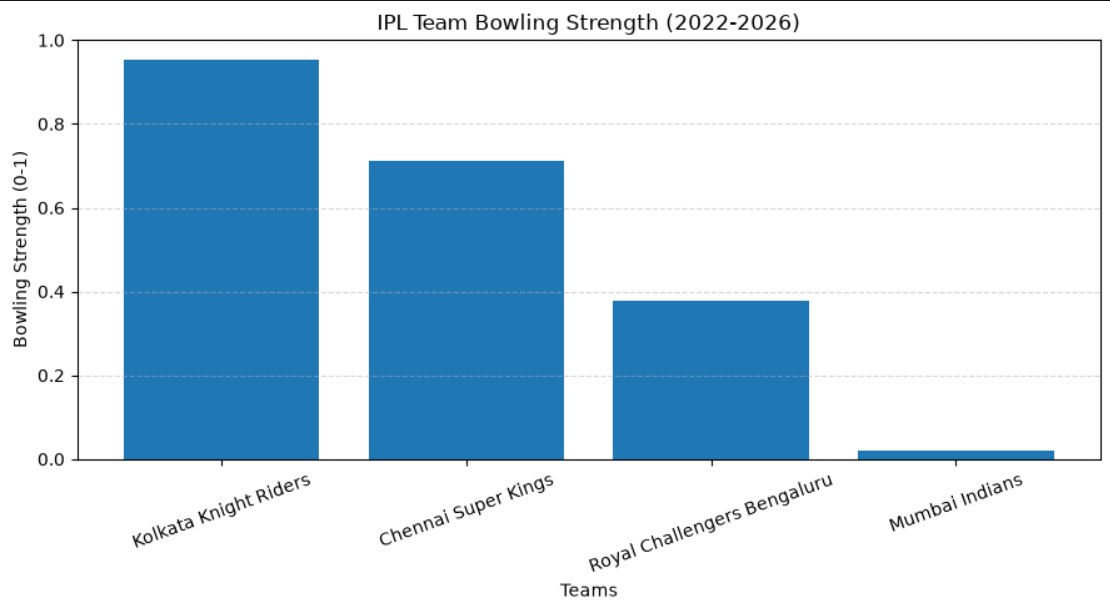
\includegraphics[width=0.8\textwidth]{Images/Battingcomp.png}
  \caption{IPL Batting Strength Distribution}
  \label{fig:batting_strength}
\end{figure}

\begin{figure}[htbp]
  \centering
   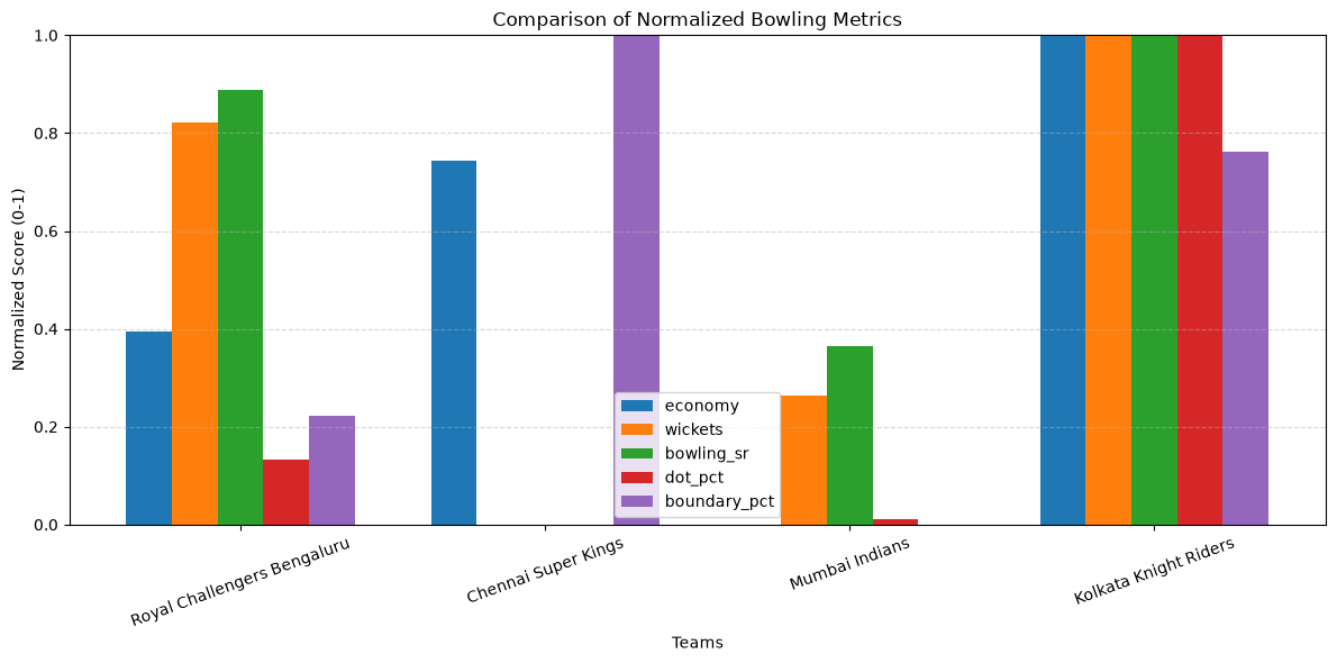
\includegraphics[width=0.8\textwidth]{Images/Bowlcomp.png}
  \caption{Bowling Metrics Comparison \& Heatmap}
  \label{fig:bowling_metrics}
\end{figure}
    \item \textbf{Home Ground Effect} :\begin{quote}
"Because playing at home naturally gives a positive advantage, we normalize the data for the home-ground team. This adjustment is why the coefficient appears negative—it ensures that every team is normalized and put on a level playing field, removing any raw bias from playing on their home pitch."
\end{quote}
    \item \textbf{Visual Artifacts:} Bar charts for team batting/bowling strengths, normalized metric comparison charts, and bowling performance heatmaps were successfully rendered in the Jupyter notebook (\texttt{a.ipynb}).
\end{itemize}

\newpage

% =====================================================================
% SECTION 3: FREQUENTLY ASKED QUESTIONS (FAQ)
% =====================================================================
\section*{Section 3: Frequently Asked Questions (FAQ)}
\addcontentsline{toc}{section}{Section 3: Frequently Asked Questions (FAQ)}

\begin{enumerate}
    \item \textbf{Q: Why use relative match scores ($Y_i$) instead of absolute runs?}  
    \textit{A:} Absolute runs are heavily biased by changing pitch conditions, impact player rules, and high-scoring inflation across different IPL years (e.g., 2008 vs. 2026). Dividing an innings score by the season average neutralizes seasonal scoring trends.
    
    \item \textbf{Q: How are neutral venues handled in the home-ground classification?}  
    \textit{A:} Venues located outside a team's recognized home stadium (e.g., UAE legs during COVID-19 or alternate host cities) are mapped to $H_i = 0$, ensuring neutral matches do not falsely inflate home advantage estimates.
    
    \item \textbf{Q: What role does Ridge Regression play in determining metric weights?}  
    \textit{A:} Ridge Regression prevents multicollinearity among correlated cricket statistics (such as strike rate and boundary percentage) and provides data-driven, objective coefficients to weight our sub-metrics.
    
    \item \textbf{Q: Why are standard errors clustered by match ID in the OLS regression?}  
    \textit{A:} Because both innings of a single match share identical weather, pitch wear, and venue characteristics, errors within the same match are correlated. Clustering by match ID corrects for this dependence.
    
    \item \textbf{Q: Does winning the toss interact with home-ground advantage?}  
    \textit{A:} While toss advantage provides tactical flexibility (choosing to bat or bowl first based on dew or pitch moisture), our regression isolates venue familiarity by controlling for team and opponent quality.
\end{enumerate}

\newpage

% =====================================================================
% SECTION 4: REFLECTION ESSAY
% =====================================================================
\section*{Section 4: Reflection Essay (Optional)}
\addcontentsline{toc}{section}{Section 4: Reflection Essay}

\subsection*{Key Takeaways and Skills Learned}
Working on this open project allowed our team to bridge theoretical data analysis concepts with real-world sports analytics. We gained hands-on proficiency in handling large-scale tabular datasets (~260,000 rows), performing complex multi-level group aggregations in Pandas, and formulating composite scoring indices that mirror professional sports franchise analytics. 

\subsection*{Broadening Beyond Standard Textbook Material}
Standard coursework often relies on clean, synthetic datasets where variables neatly align with linear assumptions. Analyzing the IPL exposed us to real-world data challenges: handling franchise name changes across 19 years, mapping unstructured stadium strings to specific home franchises, and dealing with multicollinearity in sports performance metrics. Implementing cluster-robust standard errors deepened our understanding of dependent observational data, transforming our perspective on how statistical rigor is applied to complex social and competitive environments.

\end{document}